\documentclass[tikz,border=6pt]{standalone}
\usepackage{lmodern}
\usepackage[T1]{fontenc}
\usepackage{amssymb}
\usetikzlibrary{arrows.meta,shapes.geometric,fit,backgrounds,calc,positioning}
\definecolor{letterA}{HTML}{1F5FA9}
\definecolor{letterB}{HTML}{B5651D}
\definecolor{order}{HTML}{8A9099}
\definecolor{boxline}{HTML}{B9BEC4}
\definecolor{boxfill}{HTML}{F4F5F7}
\definecolor{frozen}{HTML}{E9EEF6}
\definecolor{ref}{HTML}{A6ADB4}
\definecolor{hilite}{HTML}{DCE7F5}
\definecolor{ink}{HTML}{222629}
% Spot's LaTeX formula printer (`formula.to_str('latex')`) emits these.
\newcommand{\ttrue}{\top}
\newcommand{\ffalse}{\bot}
\newcommand{\limplies}{\rightarrow}
\newcommand{\liff}{\leftrightarrow}
\newcommand{\X}{\mathsf{X}\,}
\newcommand{\G}{\mathsf{G}\,}
\newcommand{\F}{\mathsf{F}\,}
\newcommand{\U}{\mathbin{\mathsf{U}}}
\newcommand{\W}{\mathbin{\mathsf{W}}}
\newcommand{\R}{\mathbin{\mathsf{R}}}
\newcommand{\M}{\mathbin{\mathsf{M}}}
\tikzset{
  % ---- classes and machines -------------------------------------
  cls/.style        = {circle, draw=ink, line width=.5pt, fill=white,
                       inner sep=0pt, minimum size=13mm, align=center,
                       font=\small},
  committed/.style  = {cls, double, double distance=1pt},
  entry/.style      = {draw=ink, line width=.8pt, -{Stealth[length=1.8mm]}},
  % ---- layers ----------------------------------------------------
  layerbox/.style   = {rounded corners=3pt, draw=boxline, fill=boxfill,
                       line width=.7pt},
  frozenbox/.style  = {layerbox, fill=frozen},
  layertag/.style   = {font=\scriptsize, text=ink, align=left,
                       inner sep=2pt},
  layername/.style  = {font=\scriptsize\bfseries, text=order},
  rorder/.style     = {draw=order, line width=2.2pt,
                       -{Stealth[length=3.2mm,width=3mm]}, opacity=.75},
  % ---- alphabet --------------------------------------------------
  ea/.style         = {draw=letterA, text=letterA, line width=.9pt,
                       -{Stealth[length=2mm]}},
  eb/.style         = {draw=letterB, text=letterB, line width=.9pt,
                       dashed, dash pattern=on 2.4pt off 1.6pt,
                       -{Stealth[length=2mm]}},
  eall/.style       = {draw=ink, text=ink, line width=.9pt,
                       -{Stealth[length=2mm]}},
  elab/.style       = {font=\scriptsize, inner sep=1.5pt,
                       fill=white, fill opacity=.85, text opacity=1},
  % ---- formula panels --------------------------------------------
  opnode/.style     = {rounded corners=2pt, draw=ink, fill=white,
                       line width=.5pt, inner sep=3pt, minimum height=5.5mm,
                       minimum width=9mm, font=\small, align=center},
  ophandle/.style   = {opnode, draw=order, fill=boxfill,
                       font=\footnotesize},
  opatom/.style     = {opnode, draw=letterA, text=letterA,
                       font=\small\ttfamily},
  dagedge/.style    = {draw=ink, line width=.6pt, -{Stealth[length=1.6mm]}},
  refedge/.style    = {draw=ref, line width=.5pt, densely dotted,
                       -{Stealth[length=1.4mm]}},
  slot/.style       = {font=\tiny, text=ref, inner sep=1pt, fill=white,
                       fill opacity=.85, text opacity=1},
  badge/.style      = {font=\tiny, text=order, inner sep=1pt},
  elide/.style      = {font=\scriptsize\itshape, text=order, align=center},
  panelcap/.style   = {font=\scriptsize, text=ink, align=center},
  % ---- derivation panels ------------------------------------------
  minicls/.style    = {circle, draw=order, fill=white, line width=.3pt,
                       inner sep=0pt, minimum size=3.4mm, font=\tiny,
                       text=ink},
  minibox/.style    = {rounded corners=1.4pt, draw=boxline, fill=white,
                       line width=.4pt},
  minidone/.style   = {minibox, fill=boxfill},
  minilive/.style   = {minibox, draw=letterA, fill=hilite, line width=.7pt},
  miniorder/.style  = {draw=order, line width=.9pt,
                       -{Stealth[length=1.5mm]}, opacity=.6},
  blockhead/.style  = {font=\small\bfseries, text=ink, anchor=west},
  blocknote/.style  = {font=\scriptsize\itshape, text=order, anchor=west},
  brick/.style      = {font=\small, text=ink, anchor=west},
  rulelab/.style    = {font=\scriptsize\itshape, text=order, anchor=west},
}

\begin{document}
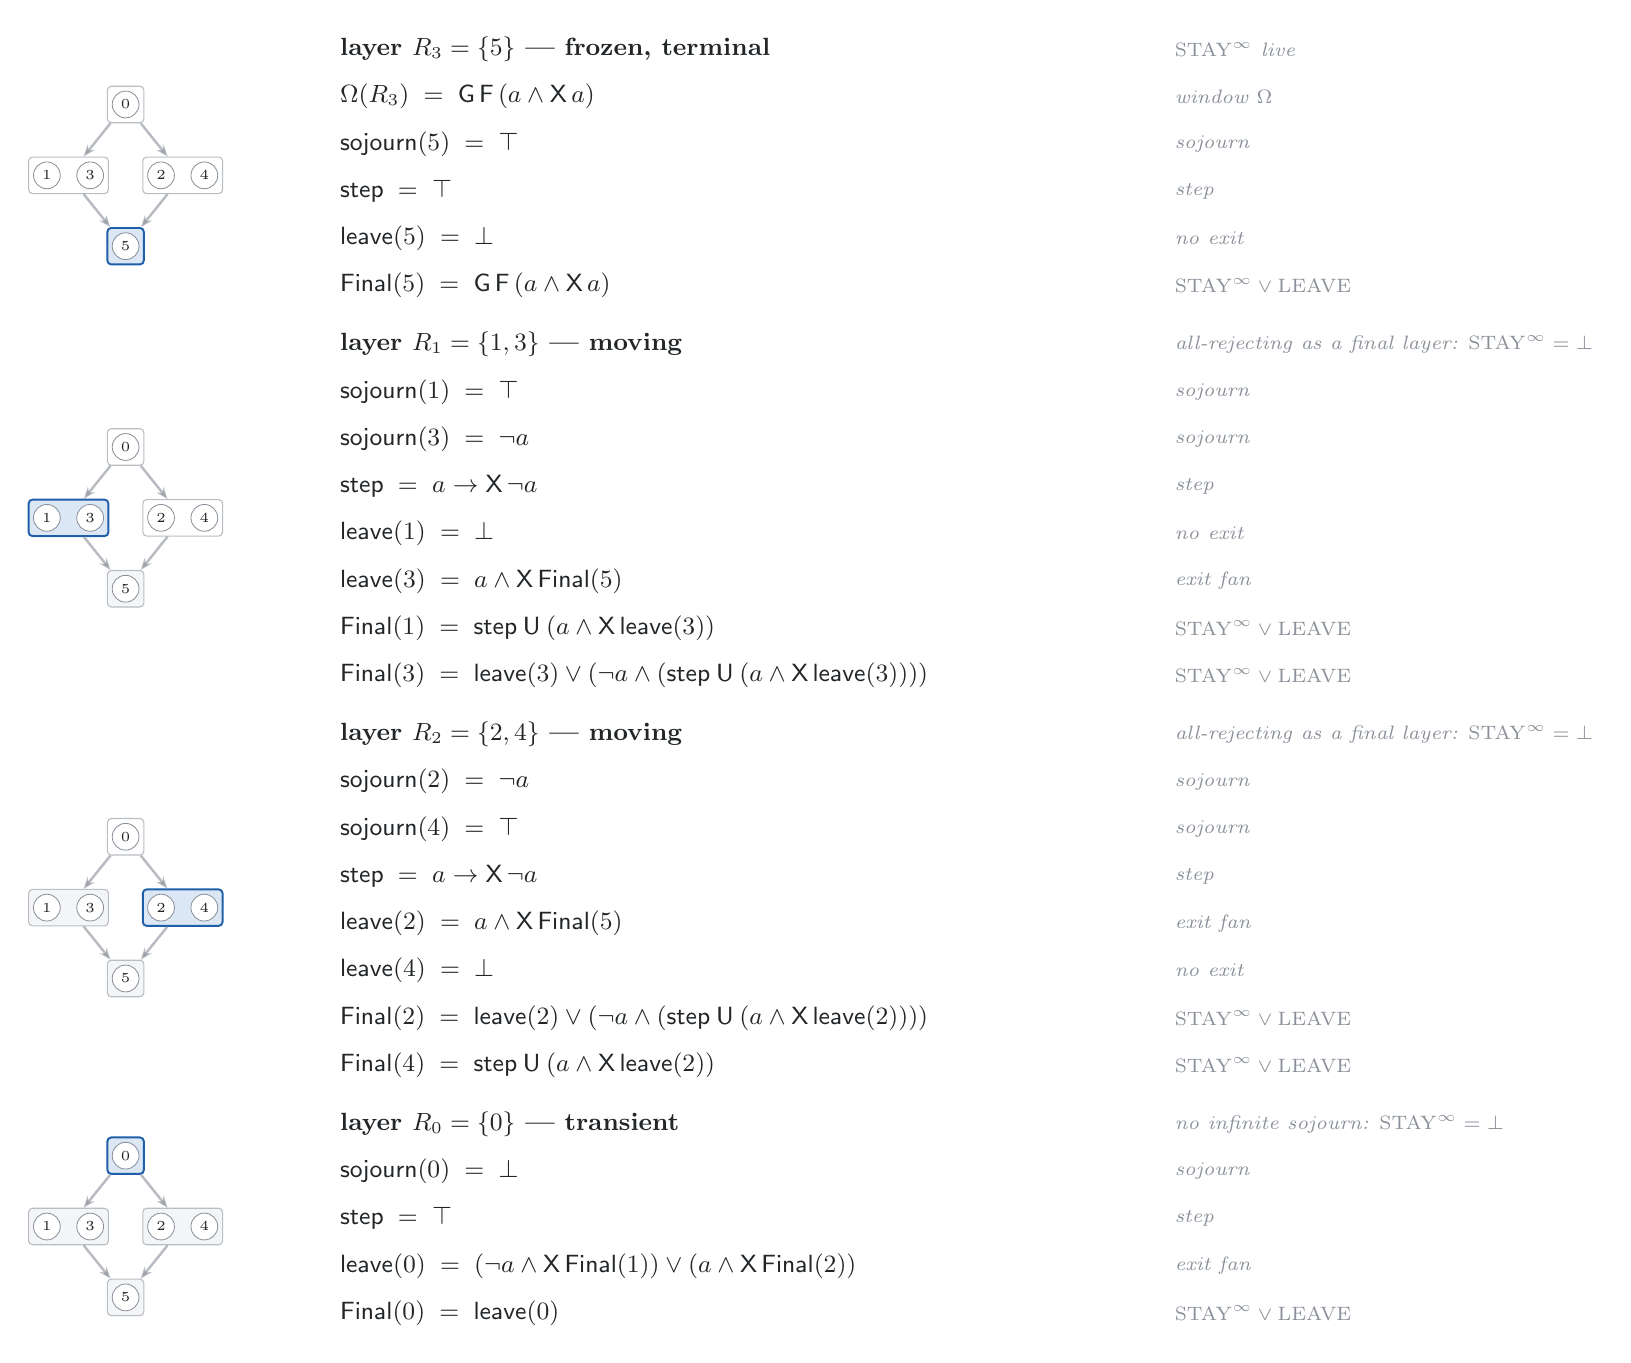
\begin{tikzpicture}
\node[blockhead] at (2.60,0.00) {layer $R_{3} = \{5\}$ --- frozen, terminal};
\node[blocknote] at (13.20,0.00) {$\mathrm{STAY}^\infty$ live};
\node[brick] at (2.60,-0.60) {$\Omega(R_{3}) \;=\; \G \F (a \land \X a)$};
\node[rulelab] at (13.20,-0.60) {window $\Omega$};
\node[brick] at (2.60,-1.20) {$\mathsf{sojourn}(5) \;=\; \ttrue$};
\node[rulelab] at (13.20,-1.20) {sojourn};
\node[brick] at (2.60,-1.80) {$\mathsf{step} \;=\; \ttrue$};
\node[rulelab] at (13.20,-1.80) {step};
\node[brick] at (2.60,-2.40) {$\mathsf{leave}(5) \;=\; \ffalse$};
\node[rulelab] at (13.20,-2.40) {no exit};
\node[brick] at (2.60,-3.00) {$\mathsf{Final}(5) \;=\; \G \F (a \land \X a)$};
\node[rulelab] at (13.20,-3.00) {$\mathrm{STAY}^\infty \lor \mathrm{LEAVE}$};
\begin{scope}[shift={(0,-0.70)}, local bounding box=m3]
  \node[minicls] (m3c0) at (0.00,0.00) {0};
  \node[minicls] (m3c1) at (-1.00,-0.90) {1};
  \node[minicls] (m3c2) at (0.45,-0.90) {2};
  \node[minicls] (m3c3) at (-0.45,-0.90) {3};
  \node[minicls] (m3c4) at (1.00,-0.90) {4};
  \node[minicls] (m3c5) at (0.00,-1.80) {5};
  \begin{scope}[on background layer]
    \node[minibox, fit=(m3c0), inner sep=1.6pt] (m3L0) {};
  \end{scope}
  \begin{scope}[on background layer]
    \node[minibox, fit=(m3c1) (m3c3), inner sep=1.6pt] (m3L1) {};
  \end{scope}
  \begin{scope}[on background layer]
    \node[minibox, fit=(m3c2) (m3c4), inner sep=1.6pt] (m3L2) {};
  \end{scope}
  \begin{scope}[on background layer]
    \node[minilive, fit=(m3c5), inner sep=1.6pt] (m3L3) {};
  \end{scope}
  \begin{scope}[on background layer]
    \draw[miniorder] (m3L0) -- (m3L1);
  \end{scope}
  \begin{scope}[on background layer]
    \draw[miniorder] (m3L0) -- (m3L2);
  \end{scope}
  \begin{scope}[on background layer]
    \draw[miniorder] (m3L1) -- (m3L3);
  \end{scope}
  \begin{scope}[on background layer]
    \draw[miniorder] (m3L2) -- (m3L3);
  \end{scope}
\end{scope}
\node[blockhead] at (2.60,-3.75) {layer $R_{1} = \{1,3\}$ --- moving};
\node[blocknote] at (13.20,-3.75) {all-rejecting as a final layer: $\mathrm{STAY}^\infty = \bot$};
\node[brick] at (2.60,-4.35) {$\mathsf{sojourn}(1) \;=\; \ttrue$};
\node[rulelab] at (13.20,-4.35) {sojourn};
\node[brick] at (2.60,-4.95) {$\mathsf{sojourn}(3) \;=\; \lnot a$};
\node[rulelab] at (13.20,-4.95) {sojourn};
\node[brick] at (2.60,-5.55) {$\mathsf{step} \;=\; a \limplies \X \lnot a$};
\node[rulelab] at (13.20,-5.55) {step};
\node[brick] at (2.60,-6.15) {$\mathsf{leave}(1) \;=\; \ffalse$};
\node[rulelab] at (13.20,-6.15) {no exit};
\node[brick] at (2.60,-6.75) {$\mathsf{leave}(3) \;=\; a \land \X \mathsf{Final}(5)$};
\node[rulelab] at (13.20,-6.75) {exit fan};
\node[brick] at (2.60,-7.35) {$\mathsf{Final}(1) \;=\; \mathsf{step} \U (a \land \X \mathsf{leave}(3))$};
\node[rulelab] at (13.20,-7.35) {$\mathrm{STAY}^\infty \lor \mathrm{LEAVE}$};
\node[brick] at (2.60,-7.95) {$\mathsf{Final}(3) \;=\; \mathsf{leave}(3) \lor (\lnot a \land (\mathsf{step} \U (a \land \X \mathsf{leave}(3))))$};
\node[rulelab] at (13.20,-7.95) {$\mathrm{STAY}^\infty \lor \mathrm{LEAVE}$};
\begin{scope}[shift={(0,-5.05)}, local bounding box=m1]
  \node[minicls] (m1c0) at (0.00,0.00) {0};
  \node[minicls] (m1c1) at (-1.00,-0.90) {1};
  \node[minicls] (m1c2) at (0.45,-0.90) {2};
  \node[minicls] (m1c3) at (-0.45,-0.90) {3};
  \node[minicls] (m1c4) at (1.00,-0.90) {4};
  \node[minicls] (m1c5) at (0.00,-1.80) {5};
  \begin{scope}[on background layer]
    \node[minibox, fit=(m1c0), inner sep=1.6pt] (m1L0) {};
  \end{scope}
  \begin{scope}[on background layer]
    \node[minilive, fit=(m1c1) (m1c3), inner sep=1.6pt] (m1L1) {};
  \end{scope}
  \begin{scope}[on background layer]
    \node[minibox, fit=(m1c2) (m1c4), inner sep=1.6pt] (m1L2) {};
  \end{scope}
  \begin{scope}[on background layer]
    \node[minidone, fit=(m1c5), inner sep=1.6pt] (m1L3) {};
  \end{scope}
  \begin{scope}[on background layer]
    \draw[miniorder] (m1L0) -- (m1L1);
  \end{scope}
  \begin{scope}[on background layer]
    \draw[miniorder] (m1L0) -- (m1L2);
  \end{scope}
  \begin{scope}[on background layer]
    \draw[miniorder] (m1L1) -- (m1L3);
  \end{scope}
  \begin{scope}[on background layer]
    \draw[miniorder] (m1L2) -- (m1L3);
  \end{scope}
\end{scope}
\node[blockhead] at (2.60,-8.70) {layer $R_{2} = \{2,4\}$ --- moving};
\node[blocknote] at (13.20,-8.70) {all-rejecting as a final layer: $\mathrm{STAY}^\infty = \bot$};
\node[brick] at (2.60,-9.30) {$\mathsf{sojourn}(2) \;=\; \lnot a$};
\node[rulelab] at (13.20,-9.30) {sojourn};
\node[brick] at (2.60,-9.90) {$\mathsf{sojourn}(4) \;=\; \ttrue$};
\node[rulelab] at (13.20,-9.90) {sojourn};
\node[brick] at (2.60,-10.50) {$\mathsf{step} \;=\; a \limplies \X \lnot a$};
\node[rulelab] at (13.20,-10.50) {step};
\node[brick] at (2.60,-11.10) {$\mathsf{leave}(2) \;=\; a \land \X \mathsf{Final}(5)$};
\node[rulelab] at (13.20,-11.10) {exit fan};
\node[brick] at (2.60,-11.70) {$\mathsf{leave}(4) \;=\; \ffalse$};
\node[rulelab] at (13.20,-11.70) {no exit};
\node[brick] at (2.60,-12.30) {$\mathsf{Final}(2) \;=\; \mathsf{leave}(2) \lor (\lnot a \land (\mathsf{step} \U (a \land \X \mathsf{leave}(2))))$};
\node[rulelab] at (13.20,-12.30) {$\mathrm{STAY}^\infty \lor \mathrm{LEAVE}$};
\node[brick] at (2.60,-12.90) {$\mathsf{Final}(4) \;=\; \mathsf{step} \U (a \land \X \mathsf{leave}(2))$};
\node[rulelab] at (13.20,-12.90) {$\mathrm{STAY}^\infty \lor \mathrm{LEAVE}$};
\begin{scope}[shift={(0,-10.00)}, local bounding box=m2]
  \node[minicls] (m2c0) at (0.00,0.00) {0};
  \node[minicls] (m2c1) at (-1.00,-0.90) {1};
  \node[minicls] (m2c2) at (0.45,-0.90) {2};
  \node[minicls] (m2c3) at (-0.45,-0.90) {3};
  \node[minicls] (m2c4) at (1.00,-0.90) {4};
  \node[minicls] (m2c5) at (0.00,-1.80) {5};
  \begin{scope}[on background layer]
    \node[minibox, fit=(m2c0), inner sep=1.6pt] (m2L0) {};
  \end{scope}
  \begin{scope}[on background layer]
    \node[minidone, fit=(m2c1) (m2c3), inner sep=1.6pt] (m2L1) {};
  \end{scope}
  \begin{scope}[on background layer]
    \node[minilive, fit=(m2c2) (m2c4), inner sep=1.6pt] (m2L2) {};
  \end{scope}
  \begin{scope}[on background layer]
    \node[minidone, fit=(m2c5), inner sep=1.6pt] (m2L3) {};
  \end{scope}
  \begin{scope}[on background layer]
    \draw[miniorder] (m2L0) -- (m2L1);
  \end{scope}
  \begin{scope}[on background layer]
    \draw[miniorder] (m2L0) -- (m2L2);
  \end{scope}
  \begin{scope}[on background layer]
    \draw[miniorder] (m2L1) -- (m2L3);
  \end{scope}
  \begin{scope}[on background layer]
    \draw[miniorder] (m2L2) -- (m2L3);
  \end{scope}
\end{scope}
\node[blockhead] at (2.60,-13.65) {layer $R_{0} = \{0\}$ --- transient};
\node[blocknote] at (13.20,-13.65) {no infinite sojourn: $\mathrm{STAY}^\infty = \bot$};
\node[brick] at (2.60,-14.25) {$\mathsf{sojourn}(0) \;=\; \ffalse$};
\node[rulelab] at (13.20,-14.25) {sojourn};
\node[brick] at (2.60,-14.85) {$\mathsf{step} \;=\; \ttrue$};
\node[rulelab] at (13.20,-14.85) {step};
\node[brick] at (2.60,-15.45) {$\mathsf{leave}(0) \;=\; (\lnot a \land \X \mathsf{Final}(1)) \lor (a \land \X \mathsf{Final}(2))$};
\node[rulelab] at (13.20,-15.45) {exit fan};
\node[brick] at (2.60,-16.05) {$\mathsf{Final}(0) \;=\; \mathsf{leave}(0)$};
\node[rulelab] at (13.20,-16.05) {$\mathrm{STAY}^\infty \lor \mathrm{LEAVE}$};
\begin{scope}[shift={(0,-14.05)}, local bounding box=m0]
  \node[minicls] (m0c0) at (0.00,0.00) {0};
  \node[minicls] (m0c1) at (-1.00,-0.90) {1};
  \node[minicls] (m0c2) at (0.45,-0.90) {2};
  \node[minicls] (m0c3) at (-0.45,-0.90) {3};
  \node[minicls] (m0c4) at (1.00,-0.90) {4};
  \node[minicls] (m0c5) at (0.00,-1.80) {5};
  \begin{scope}[on background layer]
    \node[minilive, fit=(m0c0), inner sep=1.6pt] (m0L0) {};
  \end{scope}
  \begin{scope}[on background layer]
    \node[minidone, fit=(m0c1) (m0c3), inner sep=1.6pt] (m0L1) {};
  \end{scope}
  \begin{scope}[on background layer]
    \node[minidone, fit=(m0c2) (m0c4), inner sep=1.6pt] (m0L2) {};
  \end{scope}
  \begin{scope}[on background layer]
    \node[minidone, fit=(m0c5), inner sep=1.6pt] (m0L3) {};
  \end{scope}
  \begin{scope}[on background layer]
    \draw[miniorder] (m0L0) -- (m0L1);
  \end{scope}
  \begin{scope}[on background layer]
    \draw[miniorder] (m0L0) -- (m0L2);
  \end{scope}
  \begin{scope}[on background layer]
    \draw[miniorder] (m0L1) -- (m0L3);
  \end{scope}
  \begin{scope}[on background layer]
    \draw[miniorder] (m0L2) -- (m0L3);
  \end{scope}
\end{scope}
\end{tikzpicture}
\end{document}
